\documentclass[12pt]{article}
\usepackage[utf8]{inputenc}
\usepackage{float}
\usepackage{amsmath}
\usepackage{matlab-prettifier}
\usepackage{graphicx}
\usepackage{tikz}
\usepackage{pgfplots}


\usepackage[hmargin=3cm,vmargin=6.0cm]{geometry}
%\topmargin=0cm
\topmargin=-2cm
\addtolength{\textheight}{6.5cm}
\addtolength{\textwidth}{2.0cm}
%\setlength{\leftmargin}{-5cm}
\setlength{\oddsidemargin}{0.0cm}
\setlength{\evensidemargin}{0.0cm}

%misc libraries goes here

\begin{document}

\section*{Student Information } 
%Write your full name and id number between the colon and newline
%Put one empty space character after colon and before newline
Full Name :  Aytaç SEKMEN\\
Id Number :  2575983\\

% Write your answers below the section tags
\section*{Answer 1}

\subsection*{a)}
To calculate their joint pdf and joint cdf functions, I should use the formulas given in the book:\\
$F(t_A,t_B )_{(T_A, T_B)} = P \{T_A\leq t_A \cap  T_B \leq  t_B\}$\\
Since they are "independent" and uniformly distributed events, I can rewrite it like this:\\
$F(T_A,T_B )_{(t_A, t_B)} =P \{T_A\leq t_A\}\times P \{ T_B\leq  t_B\}=F(t_A)_{(T_A)}\times F(t_B)_{(T_B)}$\\
Then by using the formula given in the book:\\
$F(t_A)_{(T_A)} = P \{ T_A \leq t_A\} =\int_{0}^{t_A} \dfrac{1}{100} \,dx =\dfrac{t_A}{100}$\\~\\
$F(t_B)_{(T_B)} = P \{ T_B \leq t_B\} =\int_{0}^{t_B} \dfrac{1}{100} \,dx =\dfrac{t_B}{100} $\\~\\
So finally I found the joint cdf funtion of $F(T_A,T_B )_{(t_A, t_B)}=\dfrac{t_A\times t_B}{10000}$\\~\\
Now I can calculate the joint pdf function by double integrating the cdf function:\\~\\
$f(t_A,t_B )_{(T_A, T_B)} = \dfrac {\partial^2}{\partial t_A \partial t_B}F(T_A,T_B )_{(t_A, t_B)}=\dfrac {\partial^2}{\partial t_A \partial t_B}\dfrac{t_A\times t_B}{10000}=\dfrac{1}{10000}$\\



%f($t_A,t_B$)=0.01 $\times$ 0.01=0.0001. And to calculate the joint cdf function I can directly use the integral formula as follows:\\
%F($t_A,t_B$)=$ \int_{0}^{t_B} \int_{0}^{t_A} \dfrac{1}{10000} \,dxdy $=$\dfrac{t_A\times t_B}{10000}$

\subsection*{b)} 
To answer this question I should consider the area as a square with each side has length 100. And I can call the x-axis as $T_A$ and y-axis as $T_B$. The small area is the area which stays between these values for $t_A$ and $t_B$:\\
$t_A\leq30$\\
$40 \leq t_B\le60$\\
And the large area is the area of square. So in my this question it asks the ratio of $\dfrac{smallarea}{largearea}$. And the ratio becomes like this: $\dfrac{20\times 30}{100\times100}$=0.06\\

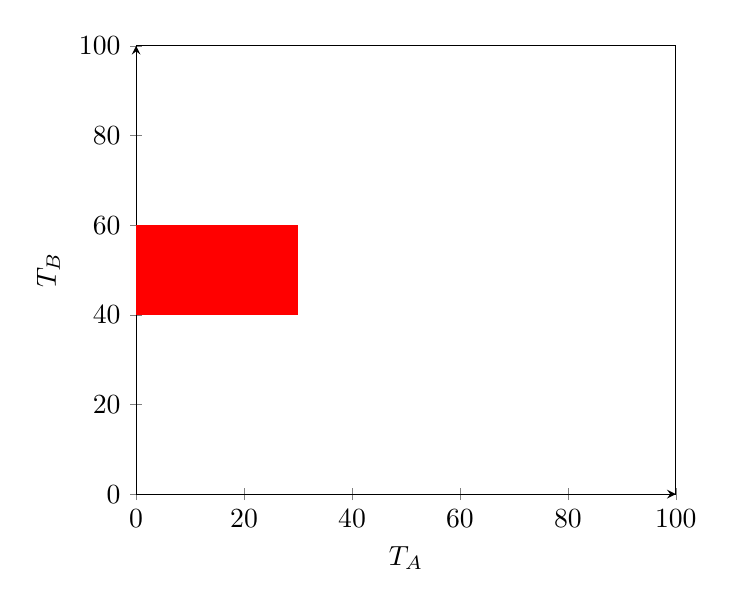
\begin{tikzpicture}
\begin{axis}[
    axis lines = left,
    xlabel = \(T_A\),
    ylabel = {\(T_B\)},
    xmin=0,
    xmax=100,
    ymin=0,
    ymax=100,
]

\draw (0, 0) rectangle (100, 100);

\fill[red] (30,40) -- (30,60) -- (0,60) --(0,40);


\end{axis}
\end{tikzpicture}



\subsection*{c)} 
We can actually model this question as follows:\\
$t_A-t_B\leq10$ which actually equals to $t_A-10\leq t_B$. So I can actually model this question as an area which stays at upper part of this line. We can think of $T_A$ is at x-axis and $T_B$ is at y axis. Since this line intersects our square at (10,0) and (100,90) our area becomes a trapezoid area which can be calculated by substracting the triangle area stays at lower-right part of the square which has the area of 4050 from the the bigger square. So if I substract this area from 10000(which is the total area of square) our probability becomes $\dfrac{smallarea}{largearea}$=$\dfrac{5950}{10000}=0.595$\\
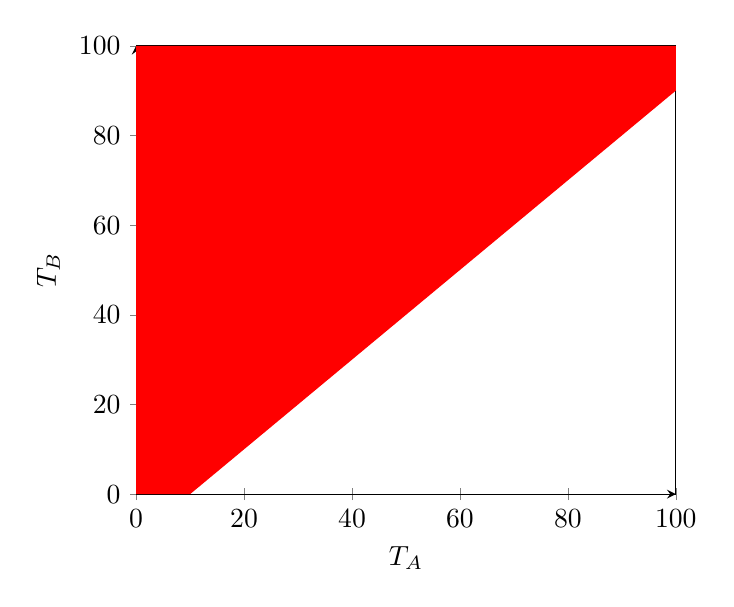
\begin{tikzpicture}
\begin{axis}[
    axis lines = left,
    xlabel = \(T_A\),
    ylabel = {\(T_B\)},
    xmin=0,
    xmax=100,
    ymin=0,
    ymax=100,
]

\draw (0, 0) rectangle (100, 100);

\fill[red] (0,0) -- (0,100) --(100,100) -- (100,90) -- (10,0)--(0,0);


\end{axis}
\end{tikzpicture}
\subsection*{d)} 
This question is actually similar to the one before. But this has 2 aspects to be considered:\\
1) $t_B\leq t_A+20$\\
2) $t_A\leq t_B+20$\\\\
Actually there is a trick in this question. One should verify that we should take the intersection area of this 2 areas, otherwise we would accept the points which we shouldn't. One area intersects the x-axis at (20,0) and other intersects y-axis at (0,20). And this 2 line are parallel to each other. To find the intersection area, we can actually find the 2 triangle areas which are at upperleft and lower-right corner. Both has the area of $\dfrac{80\times80}{2}=3200$ so in total these 2 triangle has the area of 6400. So my probability becomes: $\dfrac{smallarea}{largearea}$=$\dfrac{10000-6400}{10000}=0.36$
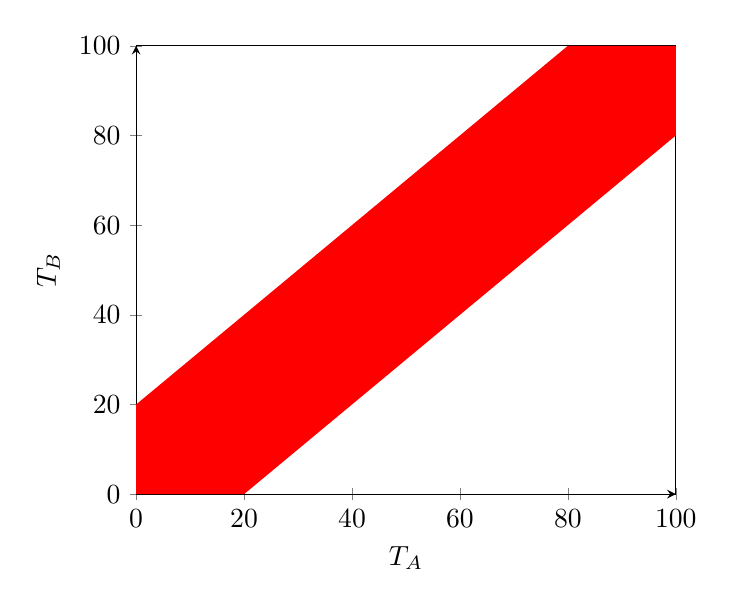
\begin{tikzpicture}
\begin{axis}[
    axis lines = left,
    xlabel = \(T_A\),
    ylabel = {\(T_B\)},
    xmin=0,
    xmax=100,
    ymin=0,
    ymax=100,
]

\draw (0, 0) rectangle (100, 100);

\fill[red] (0,0) -- (0,20) -- (80,100) --(100,100) -- (100,80) -- (20,0)--(0,0);


\end{axis}
\end{tikzpicture}


\section*{Answer 2}

\subsection*{a)} 
First of all I can consider all registered customers as a population. So the probability of a single customer to be a frequent shoppers is 0.6. So now I can actually consider the sample of 150 customers as a binomial distribution with n(number of trials)=150 and p=0.6. Since binomial distribution is a sum of individual bernoulli distribution I can apply Central Limit Theorem here, but firstly I need to calculate the expected value and the variance of this distribution.\\\\
$\mu$=$0.6\times150=90$\\
$\delta^{2}$=$0.6\times150\times0.4=36$\\
$\delta=6$\\
Also I can state that 65\% of 150 corresponds to 97.5. So I can use this as a continuity correction for the Central Limit Theorem. And this question actually asks me this "The probability that at least 98 customers in the sample are frequent shoppers.". And I can calculate this like this:\\ $P\{X\geq98\}=1-P\{X<98\}=1-P\{X<97.5\}=1-P\{\dfrac{X-\mu}{\delta}<\dfrac{97.5-90}{6}\}=1-\phi (1.25)=1- 0.8944=0.1056$ By looking at the table for Standard Normal Distribution


\subsection*{b)}
This question is really similar to the a) one.  The probability of a single customer to be a rare shoppers is 0.1. So now I can actually consider the sample of 150 customers as a binomial distribution with n(number of trials)=150 and p=0.1. Since binomial distribution is a sum of individual bernoulli distribution I can apply Central Limit Theorem here, but firstly I need to calculate the expected value and the variance of this distribution.\\\\
$\mu$=$0.1\times150=15$\\
$\delta^{2}$=$0.1\times150\times0.9=13.5$\\
$\delta\approx3.67$\\
Also I can state that 15\% of 150 corresponds to 22.5 So I can use this as a continuity correction for the Central Limit Theorem. And this question actually asks me this "The probability that no more than 22 customers in the sample are rare shoppers.". And I can calculate this like this:\\ $P\{X\leq22\}=P\{X<22.5\}=P\{\dfrac{X-\mu}{\delta}<\dfrac{22.5-15}{3.67}\}=\phi (2.04)=0.9793$ By looking at the table for Standard Normal Distribution



\section*{Answer 3}
Let me define the random variable "H" as the height of the adults. Also $\mu=175$cm and $\sigma=7cm$ So the question asks me this probability:\\\\
$P\{170< H<180\}$=$P\{\dfrac{170-175}{7}< \dfrac{H-\mu}{\delta}<\dfrac{180-175}{7}\}$=$P\{\ -0.71< Z< 0.71\}$=$\phi (0.71)$-$\phi (-0.71)$\\\\
Now when I look at the Standard Normal Distribution Table: I can see the corresponding values as 0.7611 and 0.2389 respectively. So the result is: $0.7611-0.2389\approx 0.52$

\section*{Answer 4}

\subsection*{a)}
Codes:\\
\begin{lstlisting}[style=Matlab-editor]
%datas
mu = 175;
sigma = 7;
n = 1000;
x = normrnd(mu, sigma, n, 1);

%drawing the histogram
figure('Name','Part-a','NumberTitle','off');
histogram(x);

\end{lstlisting}
Screenshot:\\
\begin{figure}[H]
  \includegraphics[width=\linewidth]{hw2_parta.png}
  \centering
  \label{fig 1:Histogram}
\end{figure}
Brief Comment:\\\\
In this code I created a histogram by creating 1000 seperate normal random variables, to resemble the graph of normal distribution. And I can actually see that this histogram resembles to normal distribution pdf function so much.
\subsection*{b)}
Codes:\\
\begin{lstlisting}[style=Matlab-editor]
%datas
mu=175;
sigma_6=6;
sigma_7=7;
sigma_8=8;

figure('Name','Part-b','NumberTitle','off');
hold on


%finding the corresponding y-values for possible x-values
x_6 = [175-28:.1:175+28];
y_6 = normpdf(x_6,mu,sigma_6);

x_7 = [175-28:.1:175+28];
y_7 = normpdf(x_7,mu,sigma_7);

x_8 = [175-28:.1:175+28];
y_8 = normpdf(x_8,mu,sigma_8);


%drawing the graphs in single plot using hold on-off calls
plot(x_6,y_6);
plot(x_7,y_7);
plot(x_8,y_8);

legend({'sigma=6','sigma=7','sigma=8'},'Location','southwest')
hold off

\end{lstlisting}
Screenshot:\\
\begin{figure}[H]
  \includegraphics[width=\linewidth]{hw2_partb.png}
  \centering
  \label{fig 2:Pdf with changing sigma values}
\end{figure}
Brief Comment:\\\\
As we can clearly see from the graph, when the $\sigma$ value increases the graph gets wider and the peak value decreases. But when the $\sigma$ decreases, the peak value increases and the graph gets narrower.
\subsection*{c)} 

Codes:\\
\begin{lstlisting}[style=Matlab-editor]
%datas
mu = 175;
sigma = 7;
n = 150;
percentages = [0.45, 0.5, 0.55];

%finding the treshold number for each percentage
thresholds = percentages * n;

%collecting the data for 1000 iterations 
number_exceed = zeros( 1,length(percentages));
for i = 1:1000
    random_variable = normrnd(mu, sigma, n, 1);
    number_in_range = sum(random_variable >= 170 & random_variable <= 180);
    number_exceed = number_exceed + (number_in_range >= thresholds);
end
probability_exceed = number_exceed / 1000;

%printing the results
for i = 1:length(probability_exceed)
    fprintf('Average for %.0f%%: %.3f\n',percentages(i)*100,probability_exceed(i));
end

\end{lstlisting}
Screenshot:\\
\begin{figure}[H]
  \includegraphics[width=\linewidth]{hw2_part4c.png}
  \centering
  \label{fig 3:Output}
\end{figure}
Brief Comment:\\\\
It is clear that the probability decreases as the desired percentage increases. And we can clearly see that the difference between average values in the range of: $45\%$-$50\%$ is smaller than the difference between the average values in the range of: $50\%$-$55\%$ even though their percentage differences are same(50-45=55-50). In addition to these, we might have slightly different average values when try to get a different output, because we are not calculating the population probabilites, we are collecting datas to calculate the sample average.

\end{document}